\documentclass[a4paper]{article}

\usepackage[T1]{fontenc}
\usepackage[italian]{babel}
\usepackage[utf8x]{inputenc}
\usepackage{graphicx}
\usepackage[margin=2.5cm]{geometry}



\begin{document}
	\title{Interferometro di Michelson}
	\maketitle
	
	\section*{To do}
	
	
	\begin{abstract}
		 Misura della lunghezza d'onda di tre diversi laser.
		 
		 Misura di spostamenti micrometrici: isteresi di un piezoelettrico.
		 
		 Misura dell'indice di rifrazione dell'aria
	\end{abstract}

\section{Teoria}
\begin{center}
	\begin{minipage}[c]{.50\textwidth}
		\centering
		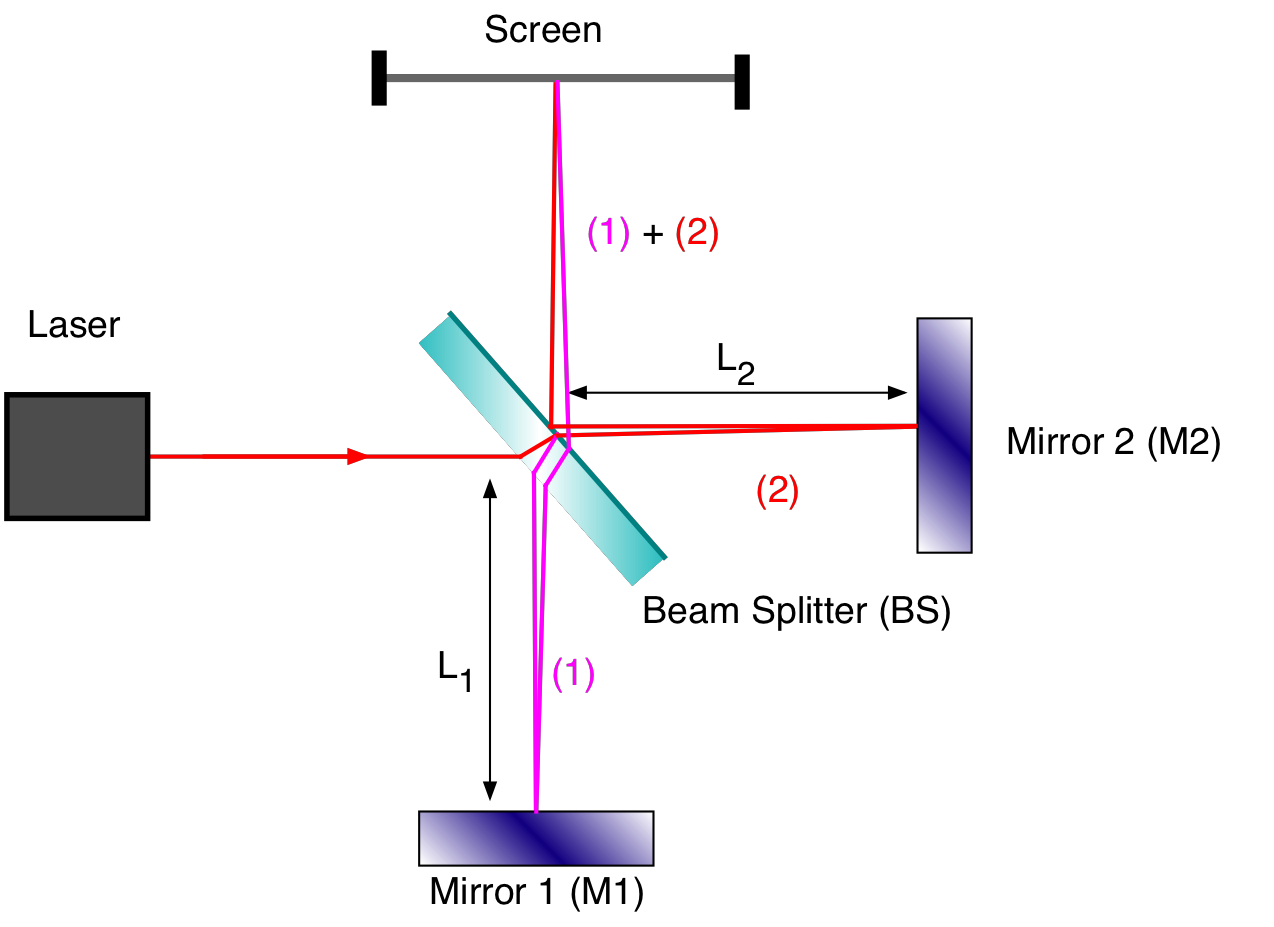
\includegraphics[width=1\textwidth]{michelson.png}
	\end{minipage}
	\begin{minipage}[c]{.40\textwidth}
		In un interferometro di Michelson come quello in figura la condizione per avere interferenza costruttiva è $2(L_1 -L_2) = m \lambda$. Nel nostro apparato contiamo il numero $m$ di frange al variare di $L_2$. 
	\end{minipage}
\end{center}

\section{Apparato sperimetale}

	Abbiamo a disposizione 
	\begin{itemize}
		\item Tre laser di diversa lunghezza d'onda: 633 nm (laser HeNe), 650 nm, 532 nm.
		\item Un interferometro di Michelson a divisione di ampiezza.
		\item Un motorino passo passo che mette in rotazione una vite micrometrica.
		\item Un rilevatore al silicio (fotodiodo) per misurare l'intensità luminosa.
		\item Una pompa a vuoto.
	\end{itemize}
Il principio di funzionamento è l'interferenza a divisione di ampiezza. Per avere interferenza al finito usiamo una lente che trasforma onde piane in onde sferiche. Le frange di interferenza vengono rivelate tramite un fotodiodo il cui segnale viene letto al PC tramite un VI labVIEW, che salva anche i dati.

\section{Misura della lunghezza d'onda}
Per misurare la lungezza d'onda del laser contiamo le frange di interferenza al variare della differenza di cammino ottico. Nell'apparato che utilizziamo lo specchio M1 è fisso mentre la distanza L2 dello specchio M2 è variata lentamente tramite una vite micrometrica azionata da un motore passo passo.
Il motorino si muove ad una velocità di 125 step/s che corrispondono ad un avanzamento della vite di circa 0.3 $\mu$m/s, quindi vediamo circa una frangia al secondo.

\section{Isteresi del piezoelettrico}

\section{Indice di rifrazione dell'aria}


\end{document}
